\documentclass[b5j,twoside,openany]{jsbook}
\usepackage[top=20truemm,bottom=20truemm,left=25truemm,right=20truemm]{geometry}
\usepackage[dvips]{color}
\usepackage[dvipdfmx]{graphicx}
\usepackage{listings,jlisting,ascmac}
\usepackage{ascmac,ulinej,url}
\usepackage{indentfirst}
\usepackage{titlesec}

\definecolor{Brown}{cmyk}{0,0.81,1,0.60}
\definecolor{OliveGreen}{cmyk}{0.64,0,0.95,0.40}
\definecolor{CadetBlue}{cmyk}{0.62,0.57,0.23,0}
\lstset{%
  language=C,
  stringstyle={\ttfamily},
  commentstyle={\itshape},
  identifierstyle={\ttfamily\color{CadetBlue}\bfseries}, 
  keywordstyle={\ttfamily\color{OliveGreen}},
  basicstyle={\ttfamily},
  breaklines=true,
  columns=[l]{fullflexible},
  frame={trbl},
  lineskip=-0.5zw,
  xrightmargin=0zw,
  xleftmargin=3zw,
  showstringspaces=ture,
  numbers={left},
  numberstyle={\scriptsize},
  stepnumber=1,
  numbersep=1zw,
  lineskip=-0.5ex,
  tabsize=1
}


% 章番号の書式の定義
\renewcommand{\thesection}{\arabic{section}}
% 横線付きsection
\newcommand{\linesection}[1]{\newpage \section{#1} \hrule width 150mm \vspace{3em}}
% ちょっと強調したい時
\newcommand{\minititle}[1]{\medskip{\large \sf #1}\medskip}

\usepackage{fancyhdr}
\pagestyle{fancy}
\lhead{}
\rhead{}
\fancyhead[RO]{\thepage{}}
\fancyhead[LE]{\thepage{}}
\cfoot{}
\renewcommand{\headrulewidth}{0pt}

\title{The book of ArchLinux}
\author{Nomuken}
\date{\today}

\begin{document}
  \linesection{はじめに}
    じぇんつーの本があるなら,あーちの本があってもいいじゃないということで書くことにしました.
    確実に他の人が既に書いている気はするのですが,近年のArchLinuxへの感謝の気持を込め,いかに使いやすいのかを伝えるために書きたいと思います.

    今回の内容は,簡単にひとまずインストール編です.次回があるのかは完全にわからないですが,デスクトップ環境にlightdm + cinnamon + mikutter環境を構築することを目標に,最速で(省略できるところは省略して)インストールを目指します.

    おそらくこの本を終えると,「極めて簡単+高速」に自分が望む環境を構築出来ることが理解していただけるものと思います.
    そして,これを読んでLinuxが必要になった時,ArchLinuxも選択肢に入れて貰えればなぁと思います.

    最後に,日々大学関係でお世話になっていて,この本の内容をギリギリまで書かずに多大なる迷惑をかけた@wakamesoba98氏に多大なる感謝を.
    あと,辛い毎日を支えてくれている,ご注文はうさぎですか??に感謝を.

    なお,表紙はArchLinuxのロゴと,フォントにKoruriを利用させていただきました.
    ちなみに,KoruriはArchLinuxだと極めて簡単にインストールでき利用できる,復数のフォントを組み合わせた美しい日本語のフォントです.\footnote{AUR ttf-koruri}

    \begin{itemize}
      \item "Archlogo" by Arch Linux Developpers - \url{http://archlinux.org/art/}
      \item "Koruri" by Hotaka Hitagi (lindwurm) - \url{http://koruri.lindwurm.biz/}
    \end{itemize}

    また,記事内ではArchLinuxの \texttrademark 表記を省略しています.

    \vspace{3em}

    なお,この文章は\url{https://spica.bz/arch-b00k/palloc_pro/document.pdf}でダウンロードすることが出来ます.
    PCからの閲覧に利用していただければと思います.
    また,2016/2/1あたりに無償公開されます,こちらも合わせてご了承ください.

  \linesection{何故ArchLinux?}
    これに関しては,多分自分が書くよりも公式のドキュメントを読むのが一番でしょう.
    \begin{itemize}
      \item ArchWiki(The Arch Way) \\ \url{https://wiki.archlinuxjp.org/index.php/The_Arch_Way}
      \item ArchWiki(Arch と他のディストリビューションの比較) \\ \url{https://wiki.archlinuxjp.org/index.php/Arch_%E3%81%A8%E4%BB%96%E3%81%AE%E3%83%87%E3%82%A3%E3%82%B9%E3%83%88%E3%83%AA%E3%83%93%E3%83%A5%E3%83%BC%E3%82%B7%E3%83%A7%E3%83%B3%E3%81%AE%E6%AF%94%E8%BC%83}
    \end{itemize}

    軽くまとめてお伝えするのであれば,ArchLinuxはユーザに常に選択を求めるディストリビューションです.
    特に,ArchLinuxではユーザが指定しなければ基本的に自分で勝手にセットアップして起動するのようなことはしません.
    そして,設定が行いやすいようにArchLinuxでは可能な限りバニラ(ArchLinux側でソースコードを改変していない)な状態でパッケージが提供されます.\footnote{ただし,Linux Kernelは2015/12/26現在patchが一つあたっています.}
    よって,ArchLinuxを利用すれば(わかっているのであれば)高速,簡単に環境を構築します.

    え?設定ファイルを書くのが大変ですか?
    安心してください,ArchLinuxはLinux界の家庭の医学とも言える恐ろしい量のパッケージセットアップの方法が記述されています.
    とても,使いやすく読みやすいのでぜひインストールにはご一読ください.\footnote{とはいえ翻訳が間に合っていないところも多く,英語版も合わせて読むことをおすすめします.例えばLXCの記事は英語のほうが参考になります.}

    ArchWikiを見ても分からないことがありましたか?
    ご安心ください,日本ではどうも人気が無いですがArchLinuxのforum\footnote{Arch Linux フォーラム - \url{https://bbs.archlinuxjp.org/}}を利用すればプロの人が教えてくれます.
    もし,あなたが英語が達者であれば活発な本流のforumを使っても良いと思いますが,日本のforumでも応答してもらえると思います.
    決して恥ずかしいと思わず,あなたが調べてどうしても分からなければ利用しても良いと思います.

    Let's ArchLinux!

  \linesection{高速にインストールしよう}
    というわけで,ArchLinuxを手短にインストールしましょう.
    おそらく,一番楽なArchLinuxの利用方法はVagrantを利用しArchLinuxのboxを入手して利用することですが,手でインストールする方法をご紹介します.
    この章を読むためには,ブラウザ等でArchLinuxのビギナーズガイドを参照しながら読むことをおすすめします.\\

    「ビギナーズガイド」\\
    \url{https://wiki.archlinuxjp.org/index.php/%E3%83%93%E3%82%AE%E3%83%8A%E3%83%BC%E3%82%BA%E3%82%AC%E3%82%A4%E3%83%89}\\

    さて,準備はできましたか?インストールしていきましょう.

    \subsection{インストールの流れ}
      インストールでは以下の条件でお話を進めます.
      \begin{itemize}
        \item GPT + BIOS環境
        \item 一番シンプルな環境
        \item lightdm + Cinnamon + mikutter環境がゴール
        \item といっても,google-chromeも使いたいよね
      \end{itemize}
      筆者の都合上,インストールはVM環境で行いながらこれを書いておりますが,
      多くの場合自分のコンピュータに入っているWindowsを抹殺してArchLinuxに入れ替えたいと思っている人も居ると思います,その場合は多分UEFI環境になります.
      冗談抜きで言えば,ArchLinuxとWindowsのデュアルブートをしたい人が主かもしれません.
      ……ここまで書いておきながら,申し訳ないのですがその人たち全員を網羅することはできません.(この本の締め切りを3回も伸ばすくらいに時間がない\footnote{@wakamesoba98氏,すみません})

      とはいえ,そのインストール方法のヒントくらいは脚注とかそんな感じで残したいと思います.
      
      そんなわけで,インストールは以下の流れで行います.
      \begin{enumerate}
        \item isoイメージで起動する
        \item 作業……その前に
        \item パーティションを分ける
        \item pacmanの設定
        \item 必要なパッケージを選ぶ
        \item 必要最低限の設定をする
          \begin{enumerate}
            \item 新環境に入る
            \item 時刻の設定
            \item 言語の設定
            \item ホスト名とネットワークの設定
            \item ユーザの設定
            \item ブートローダの設定
            \item 各種サービスの有効化
          \end{enumerate}
        \item やったぜ
      \end{enumerate}

      それでは,進めていきましょう.

    \subsection{ArchLinuxのisoイメージで起動する}
    \label{sub:ArchLinuxのisoイメージで起動する}
      isoイメージをUSBメモリに焼く方法に関しては,詳しく述べませんが以下のようなツールを使うと良いかもです.
      
      \begin{itemize}
        \item (Windows向け) dd for Windows \\ \url{http://www.si-linux.co.jp/techinfo/index.php?DD%20for%20Windows}
        \item (Mac,Linux向け) ddコマンド
      \end{itemize}
      
      そして,isoイメージから起動します.

      \begin{figure}[h!p]
        \begin{center}
          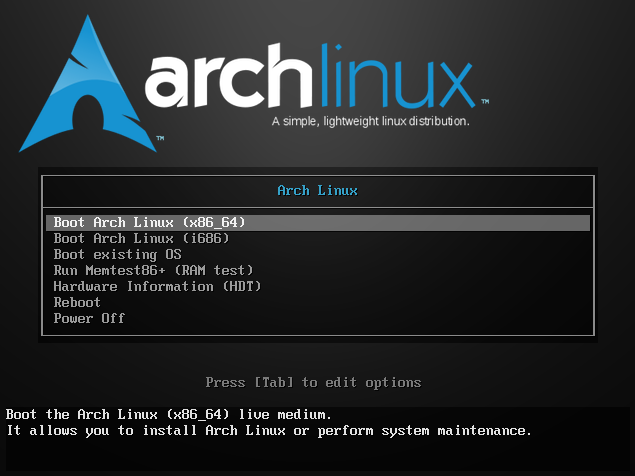
\includegraphics[width=100mm]{images/boot.png}
        \end{center}
        \caption{起動画面}
        \label{bootscreen}
      \end{figure}
      
      この時の画面を忘れないでください!
      もし,画像のように表示されたらあなたは「BIOS環境」としてArchLinuxのisoが認識しています.
      あなたがコンピュータのプロでUEFIしか許さないというなら,もう一度UEFIの設定を見なおしてください.

      もし,ArchLinuxのロゴが表示されておらず黒い画面の中にArchLinuxのブートを選ぶ画面が出ているならあなたはUEFI環境でブートしています.

    \subsection{作業……その前に}
      おっと,作業を始める前にもしあなたがjp配列のキーボードを利用しているなら以下の画面を入力してください.
      \begin{screen}
\begin{verbatim}
# loadkeys jp106
\end{verbatim}
      \end{screen}

    \subsection{パーティションを分ける}
    \label{sub:パーティションを分ける}
      パーティションを分けます.玄人の方はパーティションの構造だけで多くの時間を消費するという噂も有りますが,シンプルに考えましょう.
      今回の要件を満たすにはパーティションは2つだけで問題ありません.
      以下がその設定です.
      \begin{itemize}
        \item BIOS boot Partition(100M)
        \item その他
      \end{itemize}
      これだけで,問題ありません.
      もし,あなたがより良いパーティション構成が浮かぶのであればそちらを利用して問題ありません.
      その際には,パーティションを分け,マウントするときにマウントポイントを合わせてマウントしてください.\footnote{ビギナーズガイド 7.8.パーティションのマウント - \url{https://wiki.archlinuxjp.org/index.php/%E3%83%93%E3%82%AE%E3%83%8A%E3%83%BC%E3%82%BA%E3%82%AC%E3%82%A4%E3%83%89#.E3.83.91.E3.83.BC.E3.83.86.E3.82.A3.E3.82.B7.E3.83.A7.E3.83.B3.E3.81.AE.E3.83.9E.E3.82.A6.E3.83.B3.E3.83.88}}
      
      \begin{boxnote}
        あなたがWindowsとデュアルブートを検討している場合はここで説明される手順を行うと,Windows全てを消し飛ばしてしまいます.
        詳しくは以下の文章を参照してください.\\

        ArchWiki 「Windows と Arch のデュアルブート」\\ \url{https://wiki.archlinuxjp.org/index.php/Windows_%E3%81%A8_Arch_%E3%81%AE%E3%83%87%E3%83%A5%E3%82%A2%E3%83%AB%E3%83%96%E3%83%BC%E3%83%88} \\

        ArchLinuxとWindowsを共存させるには,まず先にWindowsをインストールしてください.
        その後ディスクの管理から,Windows領域を縮小させてからArchLinuxのISOイメージをブートしインストールすると,上手く行きます.
        ただ,その際にどこにWindows領域があるのかを忘れないようにしてください.
        UEFI環境下でWindowsとArchLinuxのデュアルブートをしようとしているなら,おそらくパーティションの2番目はEFI Boot Partitionになっているはずです.
        このパーティションを,後で/boot にマウントしてください.
      \end{boxnote}
      
      \newpage
      
      さて,パーティションを分ける前に自分のディスクがどこにマウントされているか確認しましょう.
      大体は/dev/sdaにマウントされているはずですが,時折違うところにマウントされてしまうので注意してください.
      概ね,自分が使っているSSDもしくはHDDの容量を参考に見つけると良いでしょう.
      \begin{screen}
\begin{verbatim}
# lsblk
NAME   MAJ:MIN RM   SIZE RO TYPE MOUNTPOINT
sda      8:0    0 465.8G  0 disk 
├─sda1   8:1    0   450M  0 part 
├─sda2   8:2    0    99M  0 part 
├─sda3   8:3    0    16M  0 part 
├─sda4   8:4    0  59.5G  0 part 
....skip
\end{verbatim}
      \end{screen}

      /dev/sdaのところに注目してください.
      SIZEの部分がおよそ500GB付近になっているのが解ると思います.
      このようにして,見分けることが出来ます.
      なお,本記事ではコピペによるデータ消失の悲劇を防ぐために,インストール先のディスクを/dev/sdXと表記します.

      さて,実際にパーティションを分けていきましょう.
      ここでは,パーティションを分けるためにgdiskというコマンドを利用します.
      以下の手順に従ってください.
      \begin{screen}
\begin{verbatim}
\\ Partition tableを初期化する
Command (? for help): o \\GPTで作り直し
Proceed? (Y/N): y 

\\ BIOS boot Partitionを作成する
Command (? for help): n \\パーティションを作成
Partition number (1-128, default 1): \\ defaultで良いのでEnter
First sector (34-62914526, default = 2048) or {+-}size{KMGTP}:
\\ 100M分の領域を確保する
Last sector (2048-62914526, default = 62914526) or {+-}size{KMGTP}:+100M
\\ BIOS boot Partitionを選択
Hex code or GUID (L to show codes, Enter = 8300): ef02

\\ その他のデータを格納するパーティションを作成
\\ 基本的に既定値を利用する
Command (? for help): n
Partition number (2-128, default 2): 
First sector (34-62914526, default = 206848) or {+-}size{KMGTP}: 
Last sector (206848-62914526, default = 62914526) or {+-}size{KMGTP}: 
Hex code or GUID (L to show codes, Enter = 8300): 

\\ 確認
Command (? for help): p
Number  Start (sector)  End (sector)  Size      Code Name
   1            2048        206847   100.0 MiB  EF02 BIOS boot partition
   2          206848      62914526   29.9 GiB   8300 Linux filesystem
\\ Sizeは関係なしに,Nameが同じ感じになっていればOK

\\書き込み
Command (? for help): w
Do you want to proceed? (Y/N): y
\end{verbatim}
      \end{screen}
      パーティションの操作は,難しいことが多くここで躓いてしまう人も多いかもしれません.でも,冷静に考えていけば理解は難しくないはずです.
      特に「表示されるメッセージをしっかり読む」ということを心がけるようにしましょう.
      多くのトラブルはエラー文を読めば,原因もきっと分かるはずです.原因が分かればGoogleで検索する際のキーワードも見つかりやすくなるはずです.

      \newpage

      さて,次に確保した領域をフォーマットしましょう.
      ファイルシステムに関してもbtrfsが良いなどのこだわりがある人も居たりするようらしいが,シンプルにext4でフォーマットしよう.
      先ほどの,その他の領域として構築した場所にLinuxをインストールするので先ほどのgdiskで確認した番号で言うところの2番目をフォーマットします.\footnote{忘れてしまいましたか?それならもう一度lsblkコマンドで確認してみてください,もしかしたら,lsblk -fとしたほうが分かりやすいかもしれません}
      \begin{screen}
\begin{verbatim}
# mkfs.ext4 /dev/sdX2
\end{verbatim}
      \end{screen}
      
      で,マウントします
      \begin{screen}
\begin{verbatim}
# mount /dev/sdX /mnt
\end{verbatim}
      \end{screen}
      
      \begin{boxnote}
        もし,あなたがWindowsとのデュアルブートを考えているのであれば先ほどのnoteで紹介したEFI boot Partitionをマウントすることを忘れないでください.
      \end{boxnote}

    \newpage

    \subsection{pacmanの設定}
      \subsubsection{mirrorの選択}
        この本を読んでいる人の多くは日本在住の方が多いと推定するので,ここでは日本のミラーを選択します.
        もし他のLinuxを使っていた人からするとfastmirrorのようなものが無いのかと思う人もいるかもしれません.
        一応,ArchLinuxには似たようなものとして,rankmirrorsというコマンドが有ります.これを利用すれば最速のミラーを選びmirrorlistを作成できます.\\

        「ミラー\#速度で並び替える」\\
        \url{https://wiki.archlinuxjp.org/index.php/%E3%83%9F%E3%83%A9%E3%83%BC#.E9.80.9F.E5.BA.A6.E3.81.A7.E4.B8.A6.E3.81.B3.E6.9B.BF.E3.81.88.E3.82.8B}\\

        なお,今後エディタはvimを用いて設定ファイルを編集を行っていますが,もしあなたがemacsであったりnanoであったり他のエディタを使い慣れているならそちらに置き換えて利用してください.
        なお,もしあなたがCUIで操作するエディタに慣れていないなら,nanoというエディタを利用することをおすすめします.そうするのであればvimというコマンドをnanoに置き換えて進めてください.\footnote{難しいですか?ここに操作方法が書いてあります \url{https://wiki.archlinuxjp.org/index.php/Nano#nano_.E3.81.AE.E4.BD.BF.E7.94.A8.E6.96.B9.E6.B3.95}}

         \begin{screen}
\begin{verbatim}
# vim /etc/pacman.d/mirrorlist
\\こんな感じに編集(一番上にtsukubaのミラーサーバをコピー&ペーストする)
##
## Arch Linux repository mirrorlist
## Sorted by mirror score from mirror status page
## Generated on 2015-12-01
##

Server = http://ftp.tsukuba.wide.ad.jp/Linux/archlinux/$repo/os/$arch

...skip
\end{verbatim}
        \end{screen}

      \subsubsection{multilibとarchlinuxfrの有効化}
        ArchLinuxでは,32bitライブラリが利用できるようにするには手動でmultilibというリポジトリを有効にする必要が有ります.
        結構32bitのライブラリを利用することが多いので,有効化しておきましょう.
        
        あと,ArchLinuxの最大の魅力であるAUR(ArchUserRepository) \footnote{\url{https://wiki.archlinuxjp.org/index.php/Arch_User_Repository}}とよばれる非公式ながらも任意のユーザが書いたインストールスクリプトを簡単に利用出来るようになるyaourtというコマンドも使えるようにしましょう.

        \begin{screen}
\begin{verbatim}
# vim /etc/pacman.conf
\\以下の用に編集

\\multilibの項目をコメントアウト(#を外す)
[multilib]
Include = /etc/pacman.d/mirrorlist

\\上の2つの行の下に以下を追加
[archlinuxfr]
SigLevel=Never
Server=http://repo.archlinux.fr/$arch
\end{verbatim}
        \end{screen}

        これでpacmanの設定は完了です.

    \subsection{必要なパッケージを選択する}
      初めてだと結構難しいかもしれません.冒頭で書いたゴールを具体的に振り返るとこんな感じでしょう.
      \begin{itemize}
        \item lightdm + Cinnamon + mikutter
        \item 最大限日本語で
        \item ゴールはmikutterでツイット
        \item Chromeも使いたい
        \item 今後も使えるように……
      \end{itemize}
      これらのことを踏まえると,以下のようなパッケージを入れると良いです.
      \begin{screen}
        base base-devel lightdm lightdm-gtk-greeter cinnamon nemo gnome-terminal grub networkmanager yaourt vim xorg-server xorg-server-utils mesa mesa-libgl fcitx-im fcitx-configtool fcitx-mozc
      \end{screen}
      また,GUI動作のために以下からグラフィックドライバを追加で選択してください.\footnote{詳しくはここを参照してください. \url{https://wiki.archlinuxjp.org/index.php/Xorg#.E3.83.89.E3.83.A9.E3.82.A4.E3.83.90.E3.83.BC.E3.81.AE.E3.82.A4.E3.83.B3.E3.82.B9.E3.83.88.E3.83.BC.E3.83.AB}}
      \begin{screen}
        \begin{itemize}
          \item Intel系GPUを利用 \mbox{} \\
            xf86-video-intel
          \item 最新のnvidia系GPUを利用 \mbox{} \\
            nvidia
          \item AMD系GPUを利用 \mbox{} \\
            xf86-video-ati
        \end{itemize}
      \end{screen}
      なおNVIDIAのグラフィックカードを利用している方で,とても古い4桁番台のnvidiaのグラフィックカードを使っている場合,ドライバが変わります.詳しくは次の記事を確認してください \\

      ArchWiki「NVIDIA」\\
      \url{https://wiki.archlinuxjp.org/index.php/NVIDIA} \\

      さて一気にインストールしてしまいましょう.

      \begin{boxnote}
        ここで,UEFI環境下でWindowsとデュアルブートを検討している人はブートローダを変えたほうが良いです.
        正確には,変えなくても良いのですが,個人的な感覚としてUEFI環境下のgrubはあまり適切に動作しません.
        もちろん,今後どうなるかわかりませんが,個人的にはbootctl(旧:gummiboot)を推奨しています.
        ちなみにこれは,systemdと呼ばれる必須のパッケージに組み込まれているので新たにパッケージを選ぶ必要はありません.

        また,windowsの検出にはEFIの領域を触るにはdosfstoolsというツールが必要になります.
        したがってgrubの代わりに以下のパッケージを導入してください.\\

        dosfstools
      \end{boxnote}
      \begin{boxnote}
        で,もう一個おまけです.
        もし,あなたがUEFI環境下ではなくBIOS環境下のWindowsとArchLinuxをデュアルブートをしたいならgrubを選択しつつ,
        以下のパッケージも追加でインストールしてください.これは,grubがWindowsを検知できるようにするパッケージです.\\
        os-prober
      \end{boxnote}
      以下のコマンドで環境を構築します.
      \begin{screen}
\begin{verbatim}
# pacstrap /mnt base base-devel lightdm cinnamon nemo \\
gnome-terminal grub networkmanager yaourt vim \\ 
xorg-server xorg-server-utils mesa mesa-libgl \\
fcitx-im fcitx-configtool fcitx-mozc <GPUドライバ>
\end{verbatim}
      \end{screen}
      コマンド中の$\backslash\backslash$は改行を表しています.入力せず続けて入力してください.
      コマンドを実行すると,否応無しにデフォルトパッケージがインストールされます.\footnote{実は,確認フェーズを省略するようにしてあります.もしpacstrapで確認を受けたいのであれば-iオプションをつけてインストールしてください.}
    \subsection{必要最低限の設定をする}
      \subsubsection{新環境に入る}
        まずは,新環境に入るのですがpacmanの設定を引き継ぐとともにfstabの設定をしましょう.以下のコマンドを実行してください.
        \begin{screen}
\begin{verbatim}
# cat /etc/pacman.conf > /mnt/etc/pacman.conf
# genfstab -p /mnt >> /mnt/etc/fstab
\end{verbatim}
        \end{screen}
        さて,準備は大丈夫ですね.新環境に入りましょう.
        \begin{screen}
\begin{verbatim}
# arch-chroot /mnt /bin/bash
\end{verbatim}
        \end{screen}
        実行すると新環境に移行します.\footnote{もしかしたら味気ない使いづらそうな画面だと感じたかもしれません.archisoでは,標準でzshというシェルを利用しているのに対し,新環境にはbashという一般的なシェルで入りました.もし,どうしても前のやつが良いのであれば,新環境でpacman -Syy \&\& pacman -S --noconfirm zsh grml-zsh-config \&\& zshを実行してください.}
        
      \subsubsection{時刻の設定}
        時刻の設定を行います.日本のタイムゾーンであるAsia/Tokyoを選択し,システム時計をUTCにセットします.
        \begin{screen}
\begin{verbatim}
# ln -s /usr/share/zoneinfo/Asia/Tokyo /etc/localtime
# hwclock --systohc --utc
\end{verbatim}
        \end{screen}
        \begin{boxnote}
          Windowsとデュアルブートを検討している人は注意してください.
          というのも,Windowsはlocaltime(コンピュータの時計が日本の時刻)になっているからです.
          --utcは内臓時計がutcで動いていると設定するもので,Windowsから見ると時刻がずれてしまいます.
          修正方法は,Windowsのレジストリを編集してWindowsをUTCで動作するように設定することです.詳しくはこちらを参照してください\\

          「時刻\#Windows で UTC を使う」\\
          \url{https://wiki.archlinuxjp.org/index.php/%E6%99%82%E5%88%BB#Windows_.E3.81.A7_UTC_.E3.82.92.E4.BD.BF.E3.81.86}\\

          ただ,ArchLinuxが合わせるということも出来ます.
          もし,あなたがArchLinuxをlocaltimeで動作させたいなら,--utcではなく--localtimeに変更し,
          実行してください.
        \end{boxnote}

      \subsubsection{言語の設定}
        言語の設定を行います.日本語と仮定して行いますがもしあなたが別の言語を使っているのであれば,以下のコマンドは実行せずに,エディタを利用して/etc/locale.genから自分の使っている言語をコメントアウトして保存してください.\footnote{そもそも,それが正しいやり方なのですが端折ります.その方法は次のURLを確認してください「ビギナーズガイド\#ロケール」 \url{https://wiki.archlinuxjp.org/index.php/%E3%83%93%E3%82%AE%E3%83%8A%E3%83%BC%E3%82%BA%E3%82%AC%E3%82%A4%E3%83%89#.E3.83.AD.E3.82.B1.E3.83.BC.E3.83.AB}}
        \begin{screen}
\begin{verbatim}
# echo 'en_US.UTF-8 UTF-8' >> /etc/locale.gen
# echo 'ja_JP.UTF-8 UTF-8' >> /etc/locale.gen
# locale-gen
\end{verbatim}
        \end{screen}
        また,システムが動作する言語とキーマップを指定しましょう.\footnote{もしあなたが筆者のようにUS配列以外のキーボードは使えず,US配列を利用しているユーザはecho "KEYMAP=jp106" ... のコマンドは実行しないでください.}
        \begin{screen}
\begin{verbatim}
# echo LANG=ja_JP.UTF-8 > /etc/locale.conf
# echo "KEYMAP=jp106" > /etc/vconsole.conf
\end{verbatim}
        \end{screen}

      \subsubsection{ホスト名とネットワークの設定}
        ホスト名の設定,ネットワークの設定を行います.
        \begin{screen}
\begin{verbatim}
# echo "<お好きなホスト名>" > /etc/hostname
# systemctl enable NetworkManager
\end{verbatim}
        \end{screen}
        \begin{boxnote}
          そういえば,systemctlというコマンドを利用しました.
          これは,簡単に言ってしまえば裏側で立ち上げておきたいサービスを自動起動するようにするためのコマンド
          であると,認識しておいてください.
          プロの方々には怒られてしまいそうですが,ひとまず最初はこのような認識で良いと思います.
          詳しくは,を以下の記事を確認してください.\\

          「Systemd」\\
          \url{https://wiki.archlinuxjp.org/index.php/Systemd}\\

          ところでここでは,NetworkManagerによってネットワークを管理するように設定しました.
          これは,セットアップしてるコンピュータが無線LANを利用していて,インタラクティブに設定を変更したほうが生産性が高いと判断したためです.
          しかし,有線LANのみの接続である場合はdhcpcd(\url{https://wiki.archlinuxjp.org/index.php/dhcpcd})を利用しても良いですし,
          もし,サーバのようにIPアドレスが固定でネットワークが変わらないのであれば,netctl(\url{https://wiki.archlinuxjp.org/index.php/netctl})を選択するのも良いです.
        \end{boxnote}

      \subsubsection{ユーザの設定}
        新環境で利用するユーザを作成しましょう.ここではrootのパスワードを決定し,新規ユーザの登録とパスワードの設定,そして新規ユーザがsudo(一時的な権限昇格)を許可するように設定しましょう.
        \begin{screen}
\begin{verbatim}
# passwd
Enter new UNIX password: \\入力しても表示されないが実際は入力されてる
Retype new UNIX password: 
passwd: password updated successfully

# useradd -m -g users -G wheel <ここにユーザ名>

# passwd <先ほどのユーザ名>
Enter new UNIX password: 
Retype new UNIX password: 
passwd: password updated successfully

\\ エディタにnanoを選んでるならば……
# EDITOR=nano visudo
\\ エディタにvimを選んでいるならば……
# visudo

\\ 以下の%wheel ALL=(ALL) ALLの行のコメントを外す.

...skip

## Uncomment to allow members of group wheel to execute any command
%wheel ALL=(ALL) ALL

...skip

\end{verbatim}
        \end{screen}
        これで,ユーザ作成は完了しました.
      \begin{boxnote}
        ところで,脚注で説明したzshに切り替えている人はいらっしゃいますか?
        もしかしたら,もうbashでログインはしたくないという人もいるかもしれません.
        以下のコマンドで,zshに切り替えられます.
        \begin{screen}
\begin{verbatim}
# chsh -s /bin/zsh
\end{verbatim}
        \end{screen}
        一般ユーザでもログイン後同様のコマンドを入力するとzshに切り替えられます.
        ……今頃申し訳ないかもしれないですが,useraddのコマンド時に-s /bin/zshを引数に加えることでユーザ作成時からzshにすることも出来ます.
      \end{boxnote}

    \subsubsection{ブートローダの設定}
      ブートローダの設定です.以下のようなコマンドを実行してください.
      \begin{screen}
\begin{verbatim}
# grub-install --recheck /dev/sdX
Installing for i386-pc platform.
Installation finished. No error reported.

# grub-mkconfig -o /boot/grub/grub.cfg
Generating grub configuration file ...
Found linux image: /boot/vmlinuz-linux
Found initrd image: /boot/initramfs-linux.img
Found fallback initramfs image: /boot/initramfs-linux-fallback.img
done
\end{verbatim}
      \end{screen}
      もし,エラー表示になってしまった場合は,パーティションテーブルを見なおして見てください.

      \begin{boxnote}
        もし,UEFI環境下でWindowsとデュアルブートをしているのであれば,以下のURLを参考にしてください.\\

        「ビギナーズガイド\#UEFI マザーボードの場合」\\
        \url{https://wiki.archlinuxjp.org/index.php/%E3%83%93%E3%82%AE%E3%83%8A%E3%83%BC%E3%82%BA%E3%82%AC%E3%82%A4%E3%83%89#UEFI_.E3.83.9E.E3.82.B6.E3.83.BC.E3.83.9C.E3.83.BC.E3.83.89.E3.81.AE.E5.A0.B4.E5.90.88}\\

      \end{boxnote}

    \subsubsection{各種サービスの有効化}
      お疲れ様です,あともう少し.起動時にログインマネージャが動作するように有効化しましょう.
      \begin{screen}
\begin{verbatim}
# systemctl enable lightdm
\end{verbatim}
      \end{screen}
      これで,ひとまずGUI環境は整いました.exitしてrebootしましょう!
      \begin{screen}
\begin{verbatim}
# exit
# reboot
\end{verbatim}
      \end{screen}
      なお,再起動後にusbメモリからbootするようにしている場合は解除してください.

  \subsection{やったぜ}
    ……と思ったら,上手く行っていないことに気がつくはずです.
    そう,文字が汚いし,そもそもmikutterとかをインストールしてないのです.
    由々しき問題です,すぐにインストールしましょう.
    Ctrl+Alt+Tを押すと仮想ターミナルが起動します.そちらからインストールを行いましょう.
    \begin{screen}
\begin{verbatim}
$ yaourt -S --noconfirm\\
mikutter google-chrome ttf-koruri ttf-vlgothic
Password: <一般ユーザのパスワードを入力>
\end{verbatim}
    \end{screen}
    これで準備は完了です.それではmikutterからつぶやきましょう.
    仮想ターミナルに以下のコマンドを入力してください.特に\&マークを忘れないようにしましょう.
    これが無いとターミナルを閉じた瞬間にmikutterが終了してしまいます.
    \begin{screen}
\begin{verbatim}
$ mikutter &
\end{verbatim}
    \end{screen}
    \begin{figure}[h!p]
      \begin{center}
        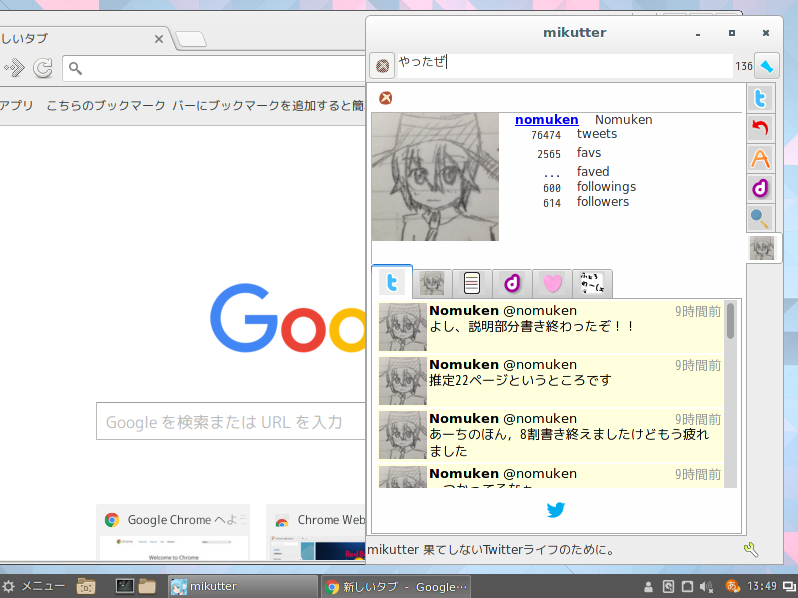
\includegraphics[width=100mm]{images/iyh.png}
      \end{center}
      \caption{インストール完了}
      \label{iyh}
    \end{figure}
    \begin{boxnote}
      昔のArchLinuxでは,fcitxの自動起動はありませんでした.
      今の自動起動はautostartにインストール後登録されすぐ使えるようになっています.
      この流れが便利かどうか,もしくは望まれることであるのかは各個人の好き嫌いがあると思います.
      それはさておき,起動しない場合はターミナルで以下のコマンドを入力してください.
      \begin{screen}
\begin{verbatim}
$ fcitx &
\end{verbatim}
      \end{screen}
      何故こんな話をするかというと,例えばxmonadやqtileのようなGNOME,KDE系でないデスクトップマネージャを利用した場合は自動起動しないためです.
    \end{boxnote}
\linesection{インストール後}
  さて,あなたは完全に動作するArchLinuxの環境を手に入れました.
  まさか,インストールを終えて満足なんてことはありませんよね?
  ArchLinuxは超便利です.100台近くある授業用のコンピュータにも,サーバにも,RaspberryPiにも使える柔軟でシンプルなLinuxです.

  もちろんWindowsの代わりとして使うことだって出来ます.
  ぜひ,もっともっとArchLinuxを使って自分にとって最も使いやすい環境を構築してください.ここから先は以下の記事が役に立つでしょう.\\

  「一般的な推奨事項」\\
  \url{https://wiki.archlinuxjp.org/index.php/一般的な推奨事項}\\

  今回は,万人受けする一般的な環境の構築を行いました.Cinnamonは美しくて綺麗なデスクトップマネージャです.
  しかし,筆者はQtileと呼ばれるデスクトップマネージャを利用しています.
  こんな具合に人それぞれの環境があります,ぜひいろんな人の環境を調べて自分の環境に取り込んでいければ良いのかなと思います.

  \subsection{パッケージマネージャyaourtの一般的な使い方}
  最後にパッケージマネージャの簡単な使い方を紹介します.
  \begin{itemize}
    \item パッケージの検索 \mbox{} \\
      yaourt $<$パッケージ名$>$
    \item パッケージのインストール \mbox{} \\
      yaourt -S $<$パッケージ名$>$
    \item パッケージの削除 \mbox{} \\
      yaourt -R $<$パッケージ名$>$
    \item パッケージの更新 \mbox{} \\
      yaourt -Syua
    \item データベースの更新 \mbox{} \\
      yaourt -Syy
  \end{itemize}
  特に,一日以上開けてArchLinuxをのパッケージをインストールしたりする場合は,データベースの更新を忘れないようにしましょう.

  もし,あなたが長期間に渡ってArchLinuxをアップデートせずキーチェックでエラーが出てしまうようなら以下のコマンドを試してみてください.
  \begin{screen}
\begin{verbatim}
$ sudo pacman -S archlinux-keyring
\end{verbatim}
  \end{screen}
\end{document}
